\chapter{Opis stanowiska INTECO CRANE}
\label{inteco_stanowisko}

\section{Stanowisko TCRANE}
\label{inteco_stanowisko_TCRANE}
Trójwymiarowy model laboratoryjnego modelu dźwigu ilustruje strukturę współczesnego 
żurawia, skutecznie odwzorowuje stosunek wielkości do maksymalnego podnoszonego 
ładunku. Obiekt jest wielowejściowym i wielowyjściowym systemem wyposażonym w dedykowane
czujniki do mierzenia przemieszczeń i kątów.\\
\indent Stanowisko laboratoryjne T-Crane posiada 5 enkoderów inkrementalnych. Trzy z nich
mierzą położenie elementów napędzanych przez silniki. Dwa z nich znajdują się na karetce
dźwigu i przedstawiają aktualne wychylenie obciążenia od pionu.

\begin{figure}[H]
    \label{Opis::TCRANE::Stanowisko}
    \centering
    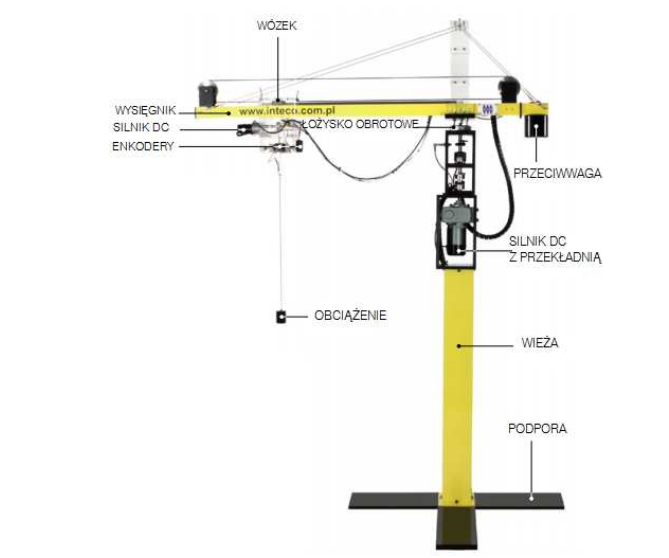
\includegraphics[scale=0.5]{./sections/inteco/images/tcrane.png}
    \caption{Stanowisko laboratoryjne TCRANE}
\end{figure}

W ramach projektu laboratoryjnego, mieliśmy wysterować ramię dźwigu w dwóch płaszczyznach:

\begin{itemize}
    \item obrót kolumny dźwigu (wieży) - oś Y
    \item ruch wózka wzdłuż ramienia - oś X
\end{itemize}



\section{Enkodery inkrementalne}
\label{inteco_stanowisko_Enkodery}
Enkoder (przetwornik położenia) służy do pomiaru położenia. W powyższej wersji
mamy do czynienia z przetwornikiem obrotowym. Zatem możemy dzięki niemu określić
położenie kątowe wokół osi. Jeżeli podłączymy go do liniowego układu przeniesienia napędu
możemy określić położenie liniowe wyrażane w odległości.\\
\indent Do określenia kierunku potrzebujemy dwóch sygnałów (tzw.
fazy A i B).Do określenia pozycji wykorzystujemy dwa wejścia do zliczania 
impulsów z fazy A i B. Wykrywanie kierunku jest wykonywane
automatycznie w sterowniku. Przy pomocy mechanizmu sprzętowych liczników możemy w
dowolnym momencie odczytać aktualne położenie enkodera. W pamięci
sterownika pozycja będzie przedstawiona w odpowiednim rejestrze 32 bitowym.\\
\indent Zliczanie impulsów odbywa się za pomocą liczników \emph{High Speed Counter}.
Pozycja zadawana w procentach jest programowo zamieniana na impulsy enkodera 
według następującego wzoru:

$$ I = \frac{STPT * MAX}{100\%}$$

Dla wózka jeżdżącego wzdłuż ramienia $$MAX_{wozek} = 9000,$$
natomiast dla wieży $$MAX_{wieza} = 2300$$

Odczyt z enkoderów inkrementalnych odbywał się za pomocą specjalnych liczników \emph{High Speed
Counter}. Skonfigurowaliśmy dwa kanały CH1 oraz CH5 do odczytu pozycji wózka oraz obrotu wieży. 
Wartość pozycji wózka odczytywaliśmy spod adresu \texttt{SD4500} a wartość pozycji kątowej wieży 
spod adresu \texttt{SD4620}.

\begin{figure}[H]
    \label{PLC::Konfiguracja::HIOEN::WindowCH1}
    \centering
    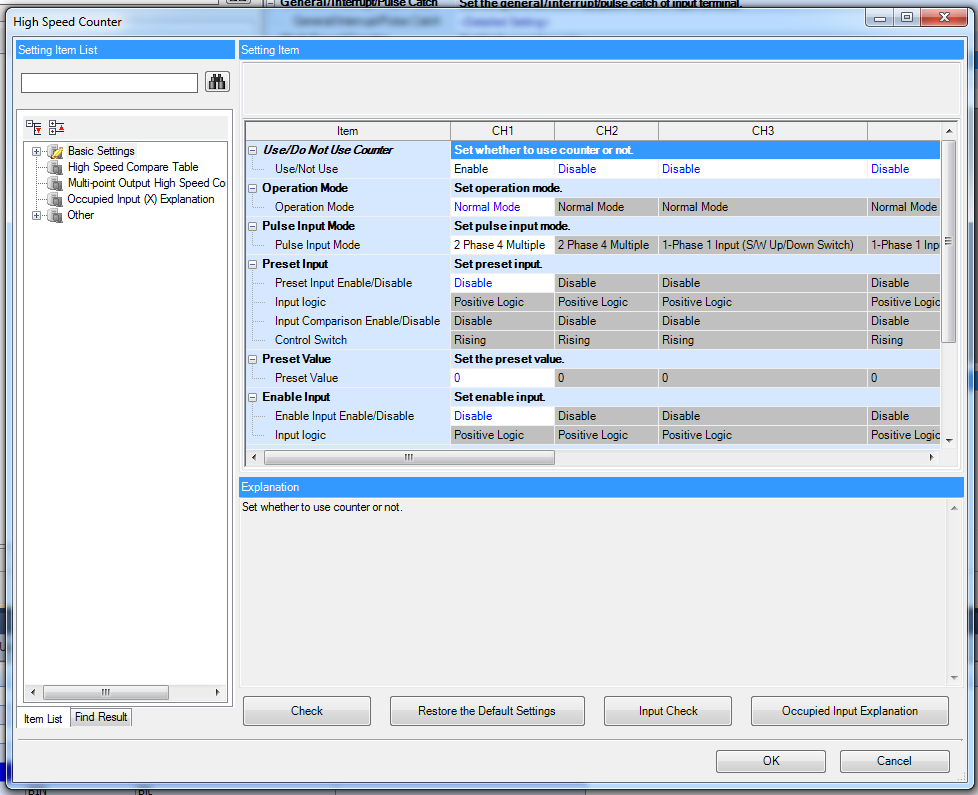
\includegraphics[scale=0.35]{./sections/inteco/images/hioen.png}
    \caption{Okno konfiguracji High Speed Counters w systemie GX Works3}
\end{figure}
\newpage

\section{Opis wejść i wyjść obiektu}
\label{Opis::IO}

Bardzo dużo czasu zajęło nam sprawdzenie który sygnał odpowiada któremu wejściu/wyjściu, 
ponieważ w dostarczonej instrukcji pojawił się błąd, mianowicie zamienione zostały sygnały 
osi wyłączników krańcowych, co wprowadziło spore zamieszanie i uniemożliwiło wykonanie zadania 
dodatkowego. Poprawny opis sygnałów wejściowych i wyjściowych znajduje się w tabelach poniżej.

\subsection{Wejścia cyfrowe}
\label{Opis::IO::Input}

\begin{table}[H]
    \centering
    \begin{tabular}{|p{0.1\linewidth}|p{0.6\linewidth}|}
	\hline
	Wejście & Opis \\ \hline
	X0 & Enkoder inkrementalny, fala A, oś X              \\ \hline
	X1 & Enkoder inkrementalny, fala B, oś X                   \\ \hline
	X2 & Enkoder inkrementalny, fala A, oś Y 		         \\  \hline
	X3 & Enkoder inkrementalny, fala B, oś Y            \\ \hline
	X4 & Enkoder inkrementalny, fala A, oś AX 		         \\  \hline
    X5 & Enkoder inkrementalny, fala B, oś AX           \\ \hline
    X6 & Enkoder inkrementalny, fala A, oś AY 		         \\  \hline
    X7 & Enkoder inkrementalny, fala B, oś AY            \\ \hline
    X10 & Enkoder inkrementalny, fala A, oś Z  		         \\  \hline
    X11 & Enkoder inkrementalny, fala B, oś Z            \\ \hline
    X12 & Wyłącznik krańcowy, oś Y 		         \\  \hline
    X13 & Wyłącznik krańcowy, oś X 		         \\  \hline
    X14 & Wyłącznik krańcowy, oś Z 		         \\  \hline
    X15 & Flaga limitu temperatury, oś Z 		         \\  \hline
    X16 & Flaga limitu temperatury, oś Y 		         \\  \hline
    X17 & Flaga limitu temperatury, oś X 		         \\  \hline
	\end{tabular}
    \caption{Wejścia instalacji INTECO TCRANE}
\end{table}

\subsection{Wyjścia cyfrowe}
\label{Opis::IO::Output}

\begin{table}[H]
    \centering
    \begin{tabular}{|p{0.1\linewidth}|p{0.6\linewidth}|}
	\hline
    Wejście & Opis \\ \hline
    Y0 & Sygnał PWM dla silnika DC, oś X  \\  \hline
	Y1 & Sygnał PWM dla silnika DC, oś Z  \\ \hline
	Y2 & Sygnał PWM dla silnika DC, oś Y  \\ \hline
	Y3 & Hamulec silnika DC, oś Z 		  \\  \hline
	Y4 & Wybór kierunku obrotów silnika DC, oś Z         \\ \hline
	Y5 & Hamulec silnika DC, oś Y 		  \\  \hline
	Y6 & Wybór kierunku obrotów silnika DC, oś Y         \\ \hline
    Y7 & Hamulec silnika DC, oś X 		  \\  \hline
    Y10 & Wybór kierunku obrotów silnika DC, oś X         \\ \hline
	\end{tabular}
	\caption{Wyjścia instalacji INTECO TCRANE}
\end{table}


\subsection{Wyjścia PWM}
\label{PLC::Konfiguracja::PWM}
Sterownanie silnikami odbywało się za pomocą wyjść cyfrowych przy użyciu PWM. PWM czyli \emph{Pulse Width Modulation} to 
technika przybliżania sygnału analogowego poprzez sygnał prostokątny o zmiennym wypełnieniu. W projekcie,
w ten sposób sterowaliśmy silnikami prądu stałego obiektu. W programie GX Works3 odpowiednio
skonfigurowaliśmy 3 kanały PWM do współpracy z trzema silnikami obiektu. Do dalszej pracy 
wykorzystaliśmy tylko dwa z nich. Kanał \emph{CH1} służył do sterowania wyciągnikiem, kanał \emph{CH2}
sterował silnikiem wózka a kanał \emph{CH3} zajmował się sterowaniem silnika obracającym wieżą.

\newpage

\begin{figure}[h]
    \label{PLC::Konfiguracja::HIOEN::WindowCH5}
    \centering
    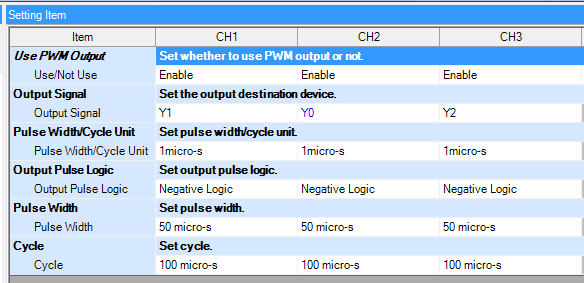
\includegraphics[scale=0.58]{./sections/inteco/images/pwm.png}
    \caption{Okno konfiguracji kanałów PWM w systemie GX Works3}
\end{figure}


\section{Komunikacja z komputerem przez port szeregowy}
\label{inteco_matlab}
Korzystając z dostarczonego szkieletu projektu, skonfigurowaliśmy komunikację z komputerem
przez port szeregowy, tak aby odczytywać dane procesowe w Matlabie. Zdecydowaliśmy się 
na zmianę okresu próbkowania z $\num{4}$s na $\num{0.5}$s tak aby lepiej dopasować regulator
do dynamiki obiektu. Aby wysyłać dane procesowe co okres próbkowania musieliśmy zmienić 
zegar taktujący z \texttt{SM412} na \texttt{SM415}. Jest to konfigurowalny licznik, który 
pozwala na ustawienie odpowiedniej liczby milisekund jako okres. Aby uzyskać żądany okres
wpisaliśmy do rejestru \texttt{SD415} wartość $\num{250}$.

\section{Konfiguracja przerwań}
\label{inteco_interrupts}
W celu uzyskania okresu próbkowania równego $T_{\mathrm{p}} = \num{0.5}$s skonfigurowaliśmy
przerwania tak aby sekcja Fixed Scan obliczała sterowania co żądany kwant czasu. W tym celu
ustawiliśmy Interrupt Setting from Internal Timer dla przerwania I31 Nna $\num{500}$ms.


\begin{figure}[h]
    \label{PLC::Konfiguracja::HIOEN::WindowCH5}
    \centering
    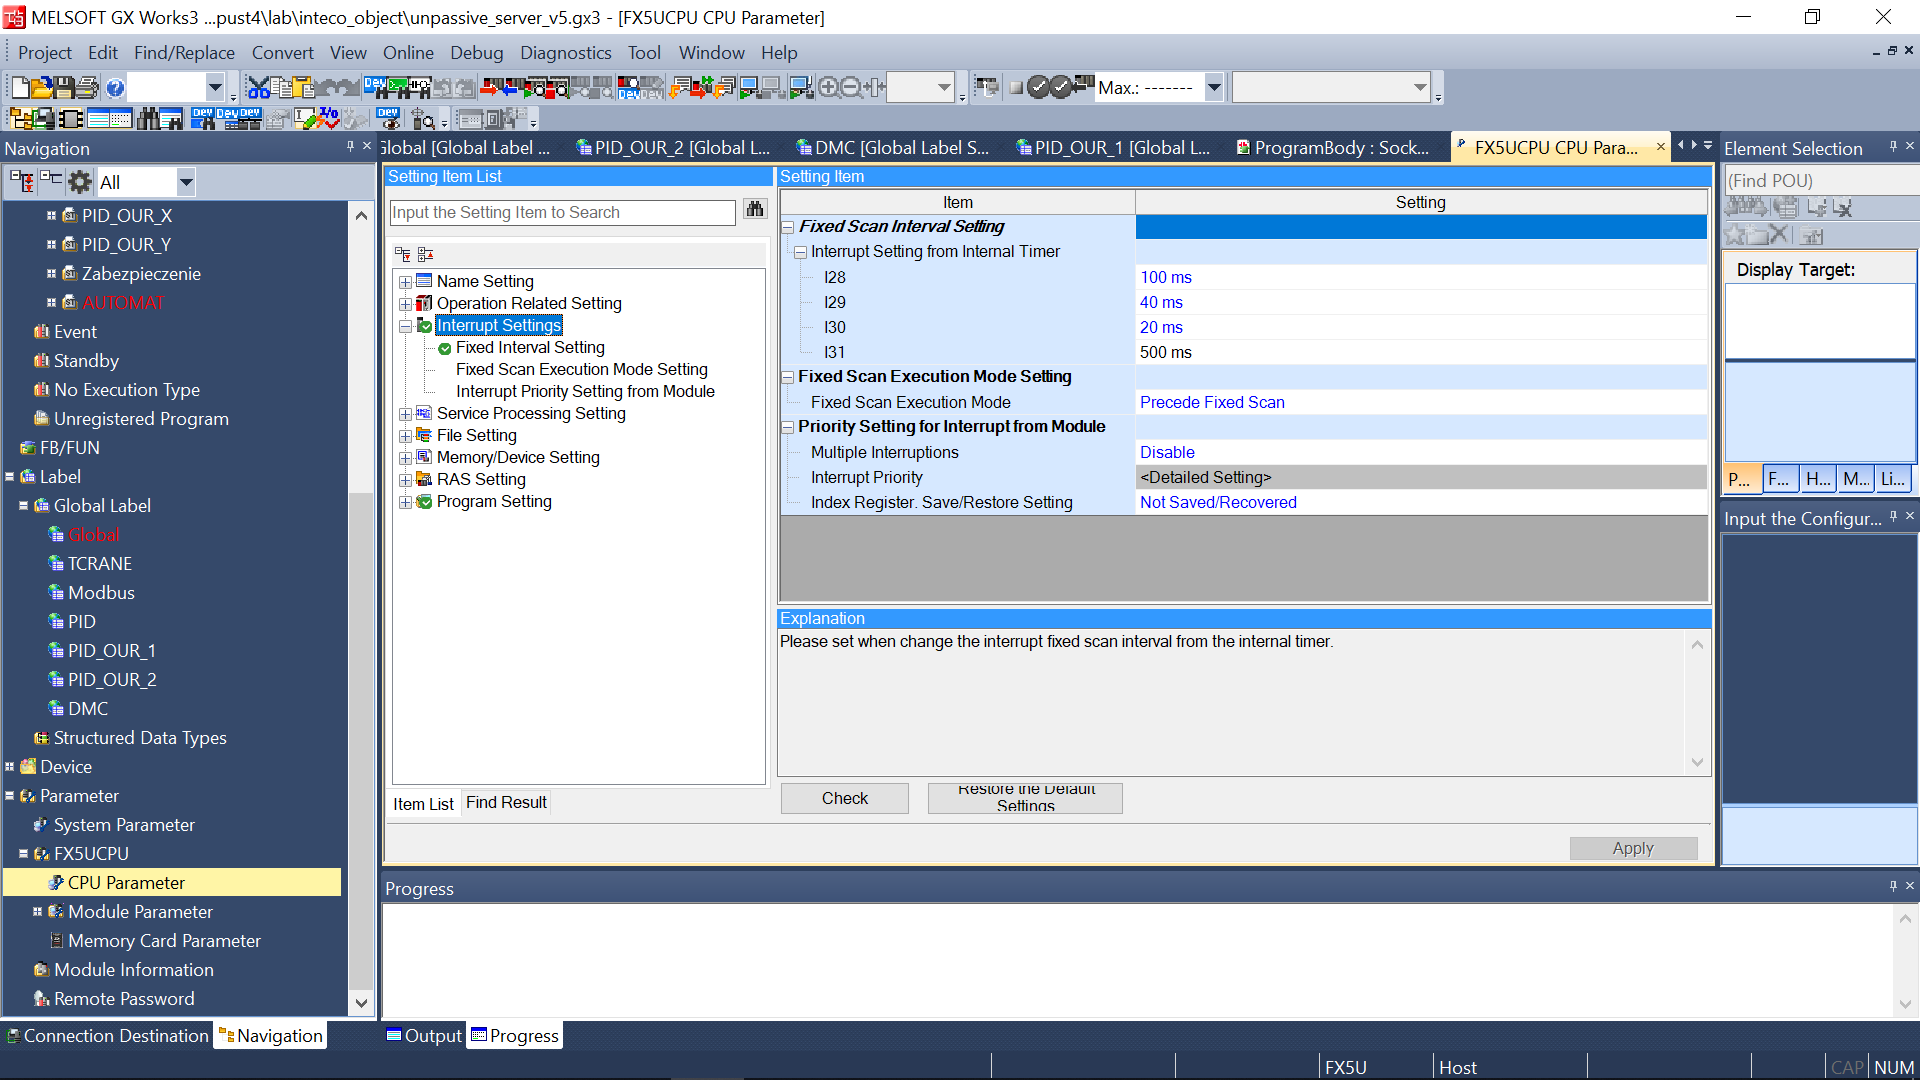
\includegraphics[scale=0.36]{./sections/inteco/images/interrupt.png}
    \caption{Konfiguracja przerwań w systemu GxWorks 3}
\end{figure}


\section{Ethernet}
\label{PLC::Konfiguracja::Ethernet}
W celu umożliwienia komunikacji sterownika z komputerem PC, wykorzystaliśmy odpowiednio 
skonfigurowane
połączenie w sieci Ethernet. Komunikacja odbywa się za pomocą protokołu SLMP (SeamLess 
Message Protocol) na porcie 1280. 

\begin{figure}[H]
    \label{PLC::Konfiguracja::Ethernet::Window}
    \centering
    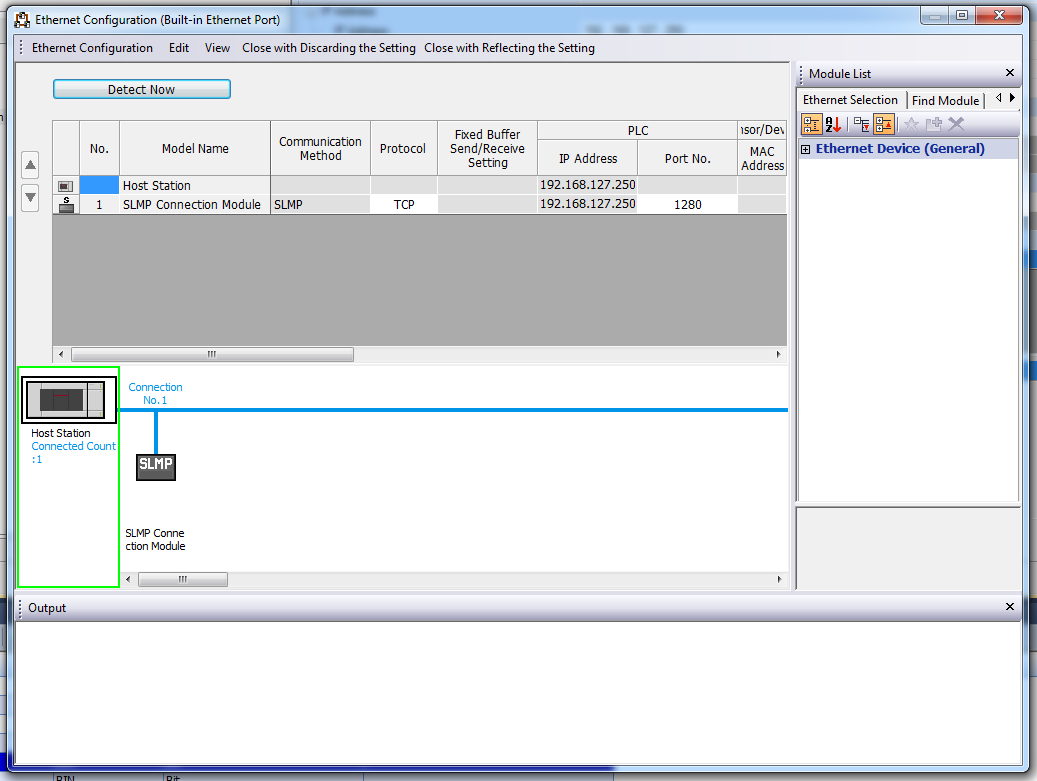
\includegraphics[scale=0.3]{./sections/inteco/images/ethernet.png}
    \caption{Konfiguracja komunikacji w sieci Ethernet w systemie GX Works3}
\end{figure}

\section{Wyznaczanie charakterystki statycznej}
\label{inteco_char_stat}

W przypadku obiektu INTECO TCRANE nie jest możliwe wyznaczenie charakterystki 
statycznej pozycji od sterowania. Silniki stanowiska są sterowane w taki sposób
że sygnał wejściowy steruje prędkością silnika, dlatego też dla każdego niezerowego
sterowania, wyjście obiektu będzie dążyło do wartości maksymalnej (w przypadku wózka
na osi X) lub dążyło do nieskończoności (w przypadku osi Y, ewentualnie do zerwania 
kabla łączącego podstawę wieży z bazą).